%----------------------------------------------------------------------------------------
%	PACKAGES AND THEMES
%----------------------------------------------------------------------------------------
\documentclass[aspectratio=169,xcolor=dvipsnames]{beamer}
\usetheme{Simple}

\usepackage{hyperref}
\usepackage{color}
\usepackage{listings}
\usepackage{minted}
\usepackage [english,russian]{babel}
\usepackage{graphicx} % Allows including images
\usepackage{booktabs} % Allows the use of \toprule, \midrule and \bottomrule in tables



%----------------------------------------------------------------------------------------
%	TITLE PAGE
%----------------------------------------------------------------------------------------

% The title
\title[short title]{Разработка приложения \\ <<Курсы Валют>> }
\subtitle{Отчет о проектной работе по курсу <<Основы информатики и программирования>>}
\author[belenkov] {Николай Беленков}
\institute[NTU] % Your institution may be shorthand to save space
{
    % Your institution for the title page
    Институт Математики и Информационных Технологий \\
    Петрозаводский Государственный Университет
    \vskip 3pt
}
\date{11 июня 2021} % Date, can be changed to a custom date


%----------------------------------------------------------------------------------------
%	PRESENTATION SLIDES
%----------------------------------------------------------------------------------------

\begin{document}

\lstdefinestyle{customc}{
  belowcaptionskip=1\baselineskip,
  breaklines=true,
  frame=L,
  xleftmargin=\parindent,
  language=C,
  showstringspaces=false,
  basicstyle=\footnotesize\ttfamily,
  keywordstyle=\bfseries\color{blue},
  commentstyle=\itshape\color{purple},
  identifierstyle=\color{black},
  stringstyle=\color{orange},
}
\lstdefinestyle{customasm}{
  belowcaptionskip=1\baselineskip,
  frame=L,
  xleftmargin=\parindent,
  language=[x86masm]Assembler,
  basicstyle=\footnotesize\ttfamily,
  commentstyle=\itshape\color{purple},
}

\lstset{escapechar=@,style=customc}

\begin{frame}
    % Print the title page as the first slide
    \titlepage
    \end{frame}

\begin{frame}{Содержание}
    \tableofcontents
\end{frame}

\section{Введение}

\begin{frame}[fragile]{Введение}
\par В наше время связь между странами стала намного более сильной. Сейчас намного проще получить из-за границы вещь, которую не купить в вашей стране, однако отслеживать цены таким образом сложнее. Курсы валют меняются каждый день, и иногда нам необходимо знать, сколько стоил доллар США или японская иена неделю назад. Таким образом, целью данного проекта стала разработка программы, способной вывести курс валют на заданную дату согласно Центральному Банку Российской Федерации.

\end{frame}

\section{Цели и задачи проекта}
\begin{frame}[fragile]{Цели и задачи проекта}
Цель проекта: Разработать приложение для вывода курсов валют на запрошенную пользователем дату.
\newline\newline
Задачи проекта: 
%%% Пример создания списков %%%
\begin{enumerate} 
    \item Разработать функцию для скачивания файла из Интернета.
    \item Разработать модуль для парсинга полученного xml.
    \item Разработать графический интерфейс пользователя.
    \item Реализовать приложение при помощи разработанных модулей и QtWidgets.
\end{enumerate}
\end{frame}

\begin{frame}[fragile]{Реализация получения xml с сайта cbr.ru}
\begin{lstlisting}
void MainWindow::get_url(QString &line)
{
    QString url = "http://www.cbr.ru/scripts/XML_daily.asp?date_req=";
    url+=line;
    QNetworkAccessManager *manager = new QNetworkAccessManager();
    connect(manager, &QNetworkAccessManager::finished,this,&MainWindow::replyFinished);
    QUrl url2(url);
    QNetworkRequest g(url2);
    manager->get(g);
}
\end{lstlisting}
\end{frame}

\begin{frame}[fragile]{Реализация парсинга xml файла}
\begin{lstlisting}
QStringList Helper::parseXml(QXmlStreamReader &xml)
{
    QStringList values;
    while (!xml.atEnd() && !xml.hasError())
    {
        QXmlStreamReader::TokenType token = xml.readNext();
        if (token == QXmlStreamReader::StartDocument)
           continue;
        if (token == QXmlStreamReader::StartElement)
        {
            if (xml.name()=="Valute")
                values.append(parseOneItem(xml));
        }
    }
    if(values.isEmpty())
        values.append("");
    return values;
}
\end{lstlisting}
\end{frame}


\begin{frame}{Интерфейс приложения}
    \begin{figure}
        \centering
        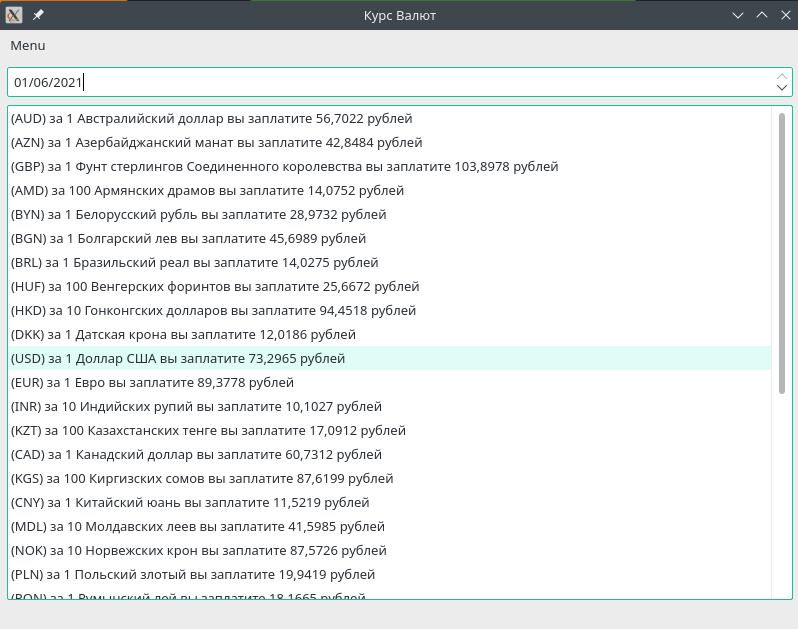
\includegraphics[scale=0.3]{interface.png}
        \caption{Интерфейс разработанного приложения}
        \label{fig:my_label}
    \end{figure}
\end{frame}

\section{Заключение}
\begin{frame}{Заключение}
В результате нам удалось разработать приложение, которое может вывести курсы валют на запрошенную пользователем дату, начиная с 1992 года и до наших дней. Программа имеет интуитивно понятный интерфейс, для взаимодействия с которым пользователю нужно всего лишь ввести интересующий его день, а программа ыведет курсы валют на этот день (или на день,в который курс обновлялся до этого). Приложение получает xml с официальных ресурсамов ЦБ РФ и выводит ответ пользователю в виде строк текста. \newline 
\parВ ходе данной работы я получил опыт работы с QtNetwork - модулем библиотеки Qt,а также с методами разбора xml файлов, опираясь на функции данной библиотеки.
\end{frame}

%----------------------------------------------------------------------------------------

\end{document}